\chapter{Series}
When writing a number with an infinite decimal, such as the Golden 
Ratio (also known as the Golden Number):
$$\phi = 1.618033988 \cdots$$

The decimal system means we can re-write the Golden Ratio (or any 
irrational number) as an infinite sum:
$$\phi = 1 + \frac{6}{10} + \frac{1}{10^2} + \frac{8}{10^3} + 
\frac{0}{10^4} + \frac{3}{10^5} + \cdots$$

You might recall from the chapter on Riemann Sums that we can 
represent the addition of many (or infinite) with big sigma notation:
$$\Sigma_{i = 1}^n a_i$$
Where i is the index as discussed in Sequences and n is the number of 
terms. For infinite sums, $n = \infty$.

\section{Partial Sums}
Let us quickly define a \textit{partial sum}. A partial sum is where 
we only look at the first $n$ terms of a series. For the general 
series, $\Sigma_{i=1}^{n} a_i$, the partial sums are:
$$s_1 = a_1$$
$$s_2 = a_1 + a_2$$
$$s_3 = a_1 + a_2 + a_3$$
$$\cdots$$
$$s_n = a_1 + a_2 + \cdots + a_n = \Sigma_{i=1}^{n} a_i$$

\textbf{Example}: A series is given by $\Sigma_{i=1}^\infty 
(\frac{-3}{4})^i$. What is the value of the partial sum $s_4$?

\textbf{Solution}: $s_4$ is the sum of the first 4 terms: 
$$(\frac{-3}{4})^1 + (\frac{-3}{4})^2 + (\frac{-3}{4})^3 + (\frac{-3}{4})^4$$
$$= \frac{-3}{4} + \frac{9}{16} + \frac{-27}{64} + \frac{81}{256} = \frac{-75}{256}$$


\section{Convergent and Divergent Series}
Just like sequences, series can also be convergent or divergent. 
Consider the series $\Sigma_{i=1}^\infty i$. Given what you already 
know about the meaning of "convergent" and "divergent", guess whether 
$\Sigma_{i=1}^\infty i$ is convergent or divergent. 

Let's determine the first few partial sums of the series (shown 
graphically in figure \ref{fig:divsum}):
\begin{center}
\begin{tabular}{|c|c|c|}\hline
n & Terms & Partial Sum\\
\hline
1 & 1 & 1\\
\hline
2 & 1+2 & 3\\
\hline
3 & 1+2+3 & 6\\
\hline
4 & 1+2+3+4 & 10\\
\hline
\end{tabular}
\end{center}

\begin{figure}[htbp]
\centering
    \begin{tikzpicture}
        \begin{axis}[axis lines = center, xmin = -0.5, xmax = 10, 
        ymin = 0, ymax = 55, xlabel=n, ylabel = $s_n$]
        \addplot[blue, mark=*](1,1);
        \addplot[blue, mark=*](2, 3);
        \addplot[blue, mark=*](3, 6);
        \addplot[blue, mark=*](4, 10);
        \addplot[blue, mark=*](5, 15);
        \addplot[blue, mark=*](6, 21);
        \addplot[blue, mark=*](7, 28);
        \addplot[blue, mark=*](8, 36);
        \addplot[blue, mark=*](9, 45);
        \addplot[blue, mark=*](10,55);
        \end{axis}
\end{tikzpicture}
    \caption{For the divergent series $\Sigma_{i=1}^n i$, the value of the 
    partial sum increases to infinity as $n$ increases}
    \label{fig:divsum}
\end{figure}

As you can see, as $n$ increases, the value of the partial sum 
increases without approaching a particular value. We can also see 
that the value of the first $n$ terms summed together is 
$\frac{n(n+1)}{2}$. This means that as $n$ approaches $\infty$, the 
sum also approaches $\infty$ and the series is divergent. 

Obviously, for a series to not become huge, the values of the terms 
should decrease as $i$ increases (that is, each subsequent term is 
smaller than the one before it). Take the series $\Sigma_{i=1}^\infty 
\frac{1}{2^i}$. As $i$ increases, $\frac{1}{2^i}$ decreases. Let's 
look at the first few partial sums of this series (shown graphically 
in figure \ref{fig:convsum}):
\begin{center}
\begin{tabular}{|c|c|c|}\hline
n & Terms & Partial Sum\\
\hline
1 & $\frac{1}{2}$ & $\frac{1}{2}$\\
\hline
2 & $\frac{1}{2} + \frac{1}{4}$ & $\frac{3}{4}$\\
\hline
3 & $\frac{1}{2} + \frac{1}{4} + \frac{1}{8}$ & $\frac{7}{8}$\\
\hline
4 & $\frac{1}{2} + \frac{1}{4} + \frac{1}{8} + \frac{1}{16}$ & 
$\frac{15}{16}$\\
\hline
\end{tabular}
\end{center}

\begin{figure}[htbp]
\centering
    \begin{tikzpicture}
        \begin{axis}[axis lines = center, xmin = -0.5, xmax = 8, 
        ymin = 0, ymax = 1.5, ytick = {1}, xlabel=n, ylabel = $s_n$]
        \addplot[blue, mark=*](1,0.5);
        \addplot[blue, mark=*](2, 3/4);
        \addplot[blue, mark=*](3, 7/8);
        \addplot[blue, mark=*](4, 15/16);
        \addplot[blue, mark=*](5, 31/32);
        \addplot[blue, mark=*](6, 63/64);
        \addplot[blue, mark=*](7, 127/128);
        \addplot[blue, mark=*](8, 255/256);
        \addplot[red, thin, dashed, domain = 0:8]{1};
        \end{axis}
\end{tikzpicture}
    \caption{For the convergent series $\Sigma_{i=1}^n \frac{1}{2^i}$, 
    the value of the partial sum approaches 1 as $n$ increases}
    \label{fig:convsum}
\end{figure}

Do you see the pattern? The $n^{th}$ partial sum is equal to 
$\frac{2^n - 1}{2^n} = 1 - \frac{1}{2^n}$. And as $n$ approaches 
$\infty$, the partial sum approaches 1. The series $\Sigma_{i=1}^\infty 
\frac{1}{2^i}$ is convergent. 

Let us define the sequence \{$s_n$\} where $s_n$ is the $n^{th}$ 
partial sum of a series:
$$s_n = \Sigma_{i=1}^n a_i$$. 

If the sequence \{$s_n$\} is convergent and $\lim_{n \to \infty} s_n$ 
exists, then the series $\Sigma_{i=1}^\infty a_i$ is also convergent. 
And if the sequence \{$s_n$\} is divergent, then the series 
$\Sigma_{i=1}^\infty a_i$ is also divergent.

\textbf{Example}: is the harmonic series, $\Sigma_{n = 1}^\infty \frac{1}{n}$ 
convergent or divergent?

\textbf{Solution}: You may think that the series is convergent, since $\lim_
{n \to \infty} \frac{1}{n} = 0$. Let's see if we can confirm this. We begin by 
looking at the partial sums $s_2$, $s_4$, $s_8$, and $s_16$:
$$s_2 = 1 + \frac{1}{2}$$
$$s_4 = 1 + \frac{1}{2} + \left(\frac{1}{3} + \frac{1}{4} \right) > 1 + 
\frac{1}{2} + \left( \frac{1}{4} + \frac{1}{4} \right) = 1 + \frac{2}{2}$$
$$s_8 = 1 + \frac{1}{2} + \left(\frac{1}{3} + \frac{1}{4} \right) + \left( 
\frac{1}{5} + \frac{1}{6} + \frac{1}{7} + \frac{1}{8} \right) > 1 + \frac{1}{2} 
+ \left(\frac{1}{4} + \frac{1}{4} \right) + \left( \frac{1}{8} + \frac{1}{8} + 
\frac{1}{8} + \frac{1}{8} \right) = 1 + \frac{3}{2}$$
$$s_{16} = 1 + \frac{1}{2} + \left(\frac{1}{3} + \frac{1}{4} \right) + \left( 
\frac{1}{5} + \frac{1}{6} + \frac{1}{7} + \frac{1}{8} \right) + \left(
\frac{1}{9} + \cdots + \frac{1}{16} \right) > $$
$$1 + \frac{1}{2} + \left(\frac{1}{4} + \frac{1}{4} \right) + \left( 
\frac{1}{8} + \frac{1}{8} + \frac{1}{8} + \frac{1}{8} \right) + \left(
\frac{1}{16} + \cdots + \frac{1}{16} \right) = 1 + \frac{4}{2}$$

Notice that, in general, $s_{2^n} > 1 + \frac{n}{2}$ for $n > 1$. Taking the 
limit as $n \to \infty$, we see that $\lim_{n \to \infty} s_{2^n} > \lim_{n 
\to \infty} 1 + \frac{n}{2} = \infty$. Therefore, $s_{2^n}$ also approaches 
$\infty$ as $n$ gets larger and the harmonic series $\Sigma_{n = 1}^\infty 
\frac{1}{n}$ is divergent. 

This example shows a very important point: the converse of a theorem is not 
always true! We do know that if a series is convergent, then the limit as n 
approaches infinity must be zero. The harmonic series shows that \textit{just 
because the limit as n approaches infinity is zero, the series is not 
necessarily convergent}. What we can say, though, is that the contrapositive 
statement is true: if the limit as n approaches infinity of a series does not 
exist or is not zero, then the series is divergent (i.e. not convergent). 

\subsection{Geometric Series}

Let's apply this definition of convergent and divergent to geometric 
series. You should recall from the chapter on sequences that a 
geometric sequence can be defined by $a_i = a(r)^{i-1}$, where $r$ 
is the common ratio and $a \neq 0$. We can express the 
\textit{geometric series} thusly:
$$a + ar + ar^2 + ar^3 = \Sigma_{i=1}^\infty ar^{i-1}$$

When are geometric series convergent? First, let's consider the case 
where $r=1$. If this is true, then $s_n = a + a + a + \cdots + a = 
na$. As $n$ approaches $\infty$, the sum will approach $\pm \infty$ 
(depending on whether $a$ is positive or negative), and the series is 
divergent. 

When $r \neq 1$, we can write $s_n$ and $rs_n$:
$$s_n = a + ar + ar^2 + \cdots + ar^{n-1}$$
$$rs_n = ar + ar^2 + ar^3 + \cdots + ar^n$$

Subtracting $rs_n$ from $s_n$, we get:
$$s_n - rs_n = (a + ar + ar^2 + \cdots + ar^{n-1}) - (ar + ar^2 + 
ar^3 + \cdots + ar^{n-1} + ar^n)$$
$$= a - ar^n$$

Solving for $s_n$, we find:
$$s_n = \frac{a(1-r^n)}{1-r}$$

We take the limit as $n \to \infty$ to determine for what values of 
$r$ the series converges:
$$\lim_{n \to \infty} s_n = \lim_{n \to \infty} \frac{a(1-r^n)}{1-r}$$
$$= \lim_{n\to \infty} \frac{a}{1-r} - \frac{ar^n}{1-r} = \frac{a}{1-r} 
- \frac{a}{1-r}\lim_{n \to \infty} r^n$$

This begs the question: when is $\lim_{n \to \infty} r^n$ convergent? 
From the sequences chapter, we know this limit converges if $|r| < 1$ 
(that is, $-1 < r < 1$). If this is true, then $\lim_{n \to \infty} 
r^n = 0$ and 
$$s_n = \frac{a}{1-r}$$

(see figures \ref{fig:geometric1} and \ref{fig:geometric2} for a visual)
\begin{figure}
    \centering
    \begin{tikzpicture}
        \begin{axis}[xmin = -0.5, xmax = 10, ymin = 0, axis lines = center, 
        xlabel = $n$, clip = false, ytick = \empty]
        \addplot[red, mark=*] (1, 2); %r=1.5
        \addplot[red, mark=*] (2, 5);
        \addplot[red, mark=*] (3, 19/2);
        \addplot[red, mark=*] (4, 65/4);
        \addplot[red, mark=*] (5, 211/8);
        \addplot[red, mark=*] (6, 665/16);
        \addplot[red, mark=*] (7, 2059/32);
        \node[red] at (5.5, 60) {$r > 1$};
        
        \addplot[orange, mark=*] (1, 2); %r=1
        \addplot[orange, mark=*] (2, 4);
        \addplot[orange, mark=*] (3, 6);
        \addplot[orange, mark=*] (4, 8);
        \addplot[orange, mark=*] (5, 10);
        \addplot[orange, mark=*] (6, 12);
        \addplot[orange, mark=*] (7, 14);
        \addplot[orange, mark=*] (8, 16);
        \addplot[orange, mark=*] (9, 18);
        \addplot[orange, mark=*] (10, 20);
        \node[orange] at (9, 25) {$r = 1$};
        
        \addplot[blue, mark =*] (1, 2); %r = 0.5
        \addplot[blue, mark =*] (2, 3);
        \addplot[blue, mark =*] (3, 7/2);
        \addplot[blue, mark =*] (4, 15/4);
        \addplot[blue, mark =*] (5, 31/8);  
        \addplot[blue, mark =*] (6, 63/16);
        \addplot[blue, mark =*] (7, 127/32);
        \addplot[blue, mark =*] (8, 255/64);
        \addplot[blue, mark =*] (9, 511/128);
        \addplot[blue, mark =*] (10, 1023/256);
        \node[blue] at (10, 10) {$0 < r < 1$};
        \end{axis}
    \end{tikzpicture}
    \caption{Geometric sequences are divergent if $r \geq 1$}
    \label{fig:geometric1}
\end{figure}

\begin{figure}
    \centering
    \begin{tikzpicture}
        \begin{axis}[xmin = -0.5, xmax = 10, axis lines = center, 
        xlabel = $n$, clip = false, ytick = \empty]
        \addplot[red, mark=*] (1, 2); %r=-1.5
        \addplot[red, mark=*] (2, -1);
        \addplot[red, mark=*] (3, 7/2);
        \addplot[red, mark=*] (4, -13/4);
        \addplot[red, mark=*] (5, 55/8);
        \addplot[red, mark=*] (6, -133/16);
        \addplot[red, mark=*] (7, 463/32);
        %\addplot[red, mark=*] (8, -1261/64);
        %\addplot[red, mark=*] (9, 4039/128);
        %\addplot[red, mark=*] (10, -11605/256);
        \node[red] at (5, 10) {$r > 1$};
        
        \addplot[orange, mark=*] (1, 2); %r=-1
        \addplot[orange, mark=*] (2, 0);
        \addplot[orange, mark=*] (3, 2);
        \addplot[orange, mark=*] (4, 0);
        \addplot[orange, mark=*] (5, 2);
        \addplot[orange, mark=*] (6, 0);
        \addplot[orange, mark=*] (7, 2);
        \addplot[orange, mark=*] (8, 0);
        \addplot[orange, mark=*] (9, 2);
        \addplot[orange, mark=*] (10, 0);
        \node[orange] at (9, -3) {$r = -1$};
        
        \addplot[blue, mark =*] (1, 2); %r = -0.5
        \addplot[blue, mark =*] (2, 1);
        \addplot[blue, mark =*] (3, 3/2);
        \addplot[blue, mark =*] (4, 5/4);
        \addplot[blue, mark =*] (5, 11/8);  
        \addplot[blue, mark =*] (6, 21/16);
        \addplot[blue, mark =*] (7, 43/32);
        \addplot[blue, mark =*] (8, 85/64);
        \addplot[blue, mark =*] (9, 171/128);
        \addplot[blue, mark =*] (10, 341/256);
        \node[blue] at (9, 5) {$-1 < r < 0$};
        \end{axis}
    \end{tikzpicture}
    \caption{Geometric sequences are divergent if $r \leq 1$. Notice that for 
    $r = -1$, the partial sums alternate between the initial term and zero.}
    \label{fig:geometric2}
\end{figure}

\textbf{Example}: Find the sum of the geometric series given by $2 - 
\frac{2}{3} + \frac{2}{9} - \frac{2}{27} + \cdots$. 

\textbf{Solution}: The first term is $a = 2$ and each the common 
ratio is $r = \frac{-1}{3}$. Since $|r| < 1$, we know that the series 
converges. We can calculate the value of the sum using the geometric 
series formula: 
$$\Sigma_{i=1}^\infty a(r)^{i-1} = \frac{a}{1-r}$$
$$\Sigma_{i=1}^\infty 2(\frac{-1}{3})^{i-1} = \frac{2}{1-\frac{-1}{3}} = 
\frac{2}{\frac{4}{3}} = \frac{6}{4} = 1.5$$

We can confirm this graphically (see figure \ref{fig:geometric}). You 
can also write out the first several partial sequences: you should 
find the sums approach 1.5 as $n$ increases.

\begin{figure}[htbp]
\centering
    \begin{tikzpicture}
        \begin{axis}[axis lines = center, xmin = -0.5, xmax = 8, 
        ymin = -1.5, ymax = 2, xlabel=n, legend pos = south east]
        \addplot[blue, mark=*](1,2);
        \addlegendentry{$s_n$};
        \addplot[red, mark=o](1, 2);
        \addlegendentry{$a_n$};
        \addplot[blue, mark=*](2, 4/3);
        \addplot[blue, mark=*](3, 14/9);
        \addplot[blue, mark=*](4, 40/27);
        \addplot[blue, mark=*](5, 122/81);
        \addplot[blue, mark=*](6, 364/243);
        \addplot[blue, mark=*](7, 1094/729);
        \addplot[blue, mark=*](8, 3280/ 2187);
        \addplot[red, mark=o](2, -2/3);
        \addplot[red, mark=o](3, 2/9);
        \addplot[red, mark=o](4, -2/27);
        \addplot[red, mark=o](5, 2/81);
        \addplot[red, mark=o](6, -2/243);
        \addplot[red, mark=o](7, 2/729);
        \addplot[red, mark=o](8, -2/2187);
        \addplot[red, thin, dashed, domain = 0:8]{1.5};
        \end{axis}
\end{tikzpicture}
    \caption{the $n^{th}$ term and partial sums of $\Sigma_{i=1}^n 
    2(\frac{-1}{3})^{i-1}$}
    \label{fig:geometric}
\end{figure}

\section{The Integral Test}
We were able to determine the exact value of some infinite series because it 
was possible to write the $n^{th}$ partial sum, $s_n$, in terms of $n$. For 
example, we determined that the $n^{th}$ partial sum of $\Sigma_{i = 1}^n 
\frac{1}{2^i}$ is $s_n = 1 - \frac{1}{2^n}$. However, it is not always possible 
to do this. How can we estimate the value of an infinite series in cases where 
we can't explicitly write $s_n$ in terms of $n$?

Consider the series $\Sigma_{i = 1}^\infty \frac{1}{i^2}$. The first few terms 
are:
$$\Sigma_{i = 1}^\infty \frac{1}{2^i} = \frac{1}{1^2} + \frac{1}{2^2} + 
\frac{1}{3^2} + \frac{1}{4^2} + \frac{1}{5^2} + \cdots$$

The series is decreasing, but is it convergent? Let's plot this series on an 
$xy$-plane (see figure \ref{fig:invsquare1}). 

\begin{figure}[htbp]
    \centering
    \begin{tikzpicture}
        \begin{axis}[xmin = -0.25, xmax = 6, axis lines = center, xlabel = $n$, 
        ymin = 0, ymax = 1.25, ytick = \empty]
        \foreach \n in {1,...,5}{
        \addplot[red, mark=*]({\n}, {1/(\n)^2});
        }
        \end{axis}
    \end{tikzpicture}
    \caption{The first 5 terms of $\Sigma_{i = 1}^\infty \frac{1}{2^i}$}
    \label{fig:invsquare1}
\end{figure}

We can overlay the function $y = \frac{1}{2^x}$ (figure \ref{fig:invsquare2}). 
We can draw rectangles of width 1 and height $\frac{1}{x^2}$ (see figure 
\ref{fig:invsquare3}). The area of the first $n$ rectangles is equal to the 
$n^{th}$ partial sum. 

\begin{figure}[htbp]
    \centering
    \begin{tikzpicture}
        \begin{axis}[xmin = -0.25, xmax = 6, axis lines = center, 
        xlabel = $n$, ymin = 0, ymax = 1.25, ytick = \empty]
        \foreach \n in {1,...,5}{
        \addplot[red, mark=*]({\n}, {1/(\n)^2});
        }
        \addplot[blue, domain = 0.7:6] {1/x^2};
        \end{axis}
    \end{tikzpicture}
    \caption{The first 5 terms of $\Sigma_{i = 1}^\infty \frac{1}{2^i}$ lie on 
    the curve $y = \frac{1}{x^2}$}
    \label{fig:invsquare2}
\end{figure}

\begin{figure}[htbp]
    \centering
    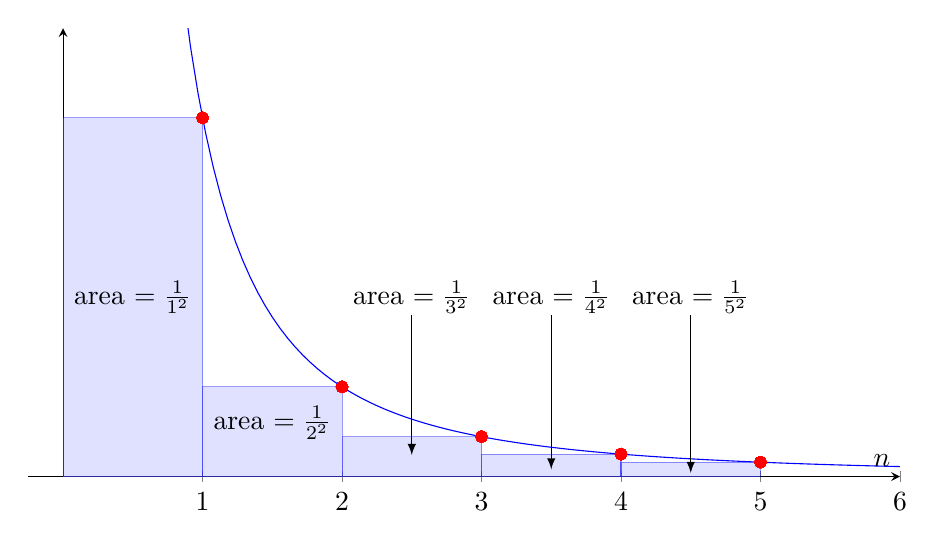
\begin{tikzpicture}
        \begin{axis}[xmin = -0.25, xmax = 6, axis lines = center, xlabel = $n$, 
        ymin = 0, ymax = 1.25, ytick = \empty, width = 1.5*\axisdefaultwidth, 
        height = \axisdefaultheight]
        \foreach \n in {1,...,5}{
        \addplot[red, mark=*]({\n}, {1/(\n)^2});
        }
        \addplot[blue, domain = 0.7:6, samples=100] {1/x^2};
        \filldraw[fill=blue!30, draw = blue, opacity = 0.4] 
        (0, 0) rectangle (1,  1);
        \filldraw[fill=blue!30, draw = blue, opacity = 0.4] 
        (1, 0) rectangle (2, 0.25);
        \filldraw[fill=blue!30, draw = blue, opacity = 0.4] 
        (2, 0) rectangle (3,  1/9);
        \filldraw[fill=blue!30, draw = blue, opacity = 0.4] 
        (3, 0) rectangle (4,  1/16);
        \filldraw[fill=blue!30, draw = blue, opacity = 0.4] 
        (4, 0) rectangle (5,  1/25);
        \node[] at (0.5, 0.5) {area $=\frac{1}{1^2}$};
        \node[] at (1.5, 0.15) {area $=\frac{1}{2^2}$};
        \node[] at (2.5, 0.5) {area $=\frac{1}{3^2}$};
        \node[] at (3.5, 0.5) {area $=\frac{1}{4^2}$};
        \node[] at (4.5, 0.5) {area $=\frac{1}{5^2}$};
        \draw[-latex](2.5, 0.45) -- (2.5, 0.06);
        \draw[-latex](3.5, 0.45) -- (3.5, 0.02);
        \draw[-latex](4.5, 0.45) -- (4.5, 0.01);
        \end{axis}
    \end{tikzpicture}
    \caption{The $5^{th}$ partial sum of $\Sigma_{i=1}^\infty \frac{1}{2^i}$ 
    is equal to the area of the rectangles}
    \label{fig:invsquare3}
\end{figure}

This should remind you of a Riemann sum. Since the total area of the rectangles 
is less than the area under the curve, we can state:
$$\Sigma_{i = 1}^\infty \frac{1}{2^i} < \int_0^\infty \frac{1}{x^2}\,dx$$

We can exclude the first rectangle and also state that: 
$$\Sigma_{i = 1}^\infty \frac{1}{2^i}< 1 + \int_1^\infty \frac{1}{x^2}\,dx$$

We can evaluate this integral:
$$\int_1^\infty \frac{1}{x^2}\,dx = \lim_{t \to \infty} \left[ \int_1^t 
\frac{1}{x^2}\,dx \right]$$
$$ = \lim_{t \to \infty} \frac{-1}{x}|_{x=1}^t = \lim_{t \to \infty} \left( 
\frac{-1}{t} \right) - \frac{-1}{1} = 0 - (-1) = 1$$

And therefore:
$$\Sigma_{i = 1}^\infty \frac{1}{2^i}< 1 + 1 = 2$$

This means the series $\Sigma_{i = 1}^\infty \frac{1}{2^i}$ is bounded above. 
Since the series is also monotonic (each term is positive, so the value of the 
sum increases as $n$ increases), we can state that the sum is convergent! 

Let's look at a divergent example: $\Sigma_{i = 1}^\infty \frac{1}{\sqrt{x}}$. 
Again, we will make a visual, but this time we will draw rectangles that lie 
above the curve $y = \frac{1}{\sqrt{x}}$ (see figure \ref{fig:invroot}). In 
this case, $\Sigma_{i = 1}^\infty \frac{1}{\sqrt{x}}> \int_1^\infty 
\frac{1}{\sqrt{x}}\,dx$. Let's evaluate the integral:
$$\int_1^\infty \frac{1}{\sqrt{x}}\,dx = \lim_{t \to \infty} \left[ \int_1^t 
\frac{1}{\sqrt{x}}\,dx \right] $$
$$= \lim_{t \to \infty} \left[ 2 \sqrt{x} \right]_{x=1}^t= \lim_{t \to \infty} 
\left( 2\sqrt{t} \right) - 2\sqrt{1} = \infty - 2 \rightarrow \text{divergent}$$

Since the integral diverges to infinity and the series is greater than the 
integral, the series must also diverge to infinity. This is another case where 
a monotonic decreasing series is not convergent!

\begin{figure}[htbp]
    \centering
    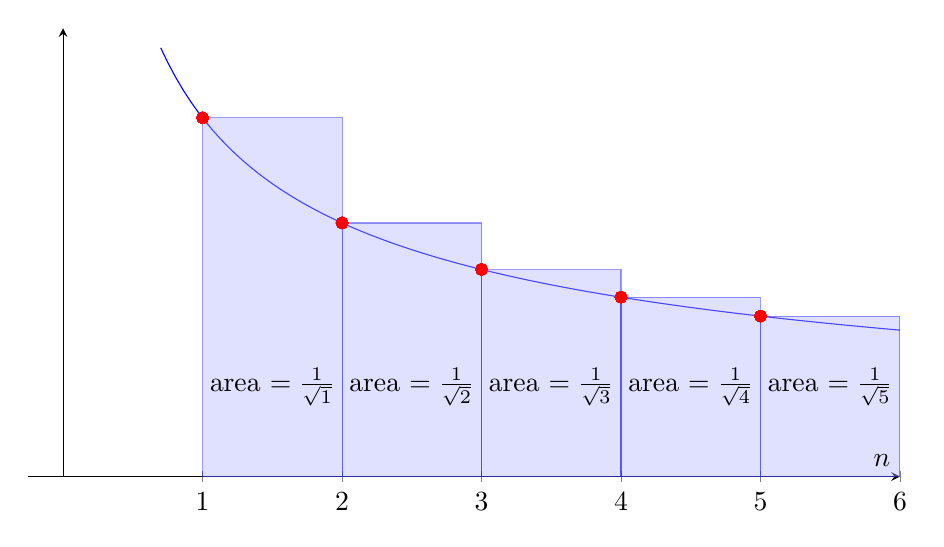
\begin{tikzpicture}
        \begin{axis}[xmin = -0.25, xmax = 6, axis lines = center, xlabel = $n$, 
        ymin = 0, ymax = 1.25, ytick = \empty, width = 1.5*\axisdefaultwidth, 
        height = \axisdefaultheight]
        \foreach \n in {1,...,5}{
        \addplot[red, mark=*]({\n}, {1/sqrt(\n)});
        }
        \addplot[blue, domain = 0.7:6, samples=100] {1/sqrt(x)};
        \filldraw[fill=blue!30, draw = blue, opacity = 0.4] 
        (1, 0) rectangle (2,  1);
        \filldraw[fill=blue!30, draw = blue, opacity = 0.4] 
        (2, 0) rectangle (3, 0.707);
        \filldraw[fill=blue!30, draw = blue, opacity = 0.4] 
        (3, 0) rectangle (4,  0.577);
        \filldraw[fill=blue!30, draw = blue, opacity = 0.4] 
        (4, 0) rectangle (5,  0.5);
        \filldraw[fill=blue!30, draw = blue, opacity = 0.4] 
        (5, 0) rectangle (6, 0.4472);
        \node[] at (1.5, 0.25) {area $=\frac{1}{\sqrt{1}}$};
        \node[] at (2.5, 0.25) {area $=\frac{1}{\sqrt{2}}$};
        \node[] at (3.5, 0.25) {area $=\frac{1}{\sqrt{3}}$};
        \node[] at (4.5, 0.25) {area $=\frac{1}{\sqrt{4}}$};
        \node[] at (5.5, 0.25) {area $=\frac{1}{\sqrt{5}}$};
        \end{axis}
    \end{tikzpicture}
    \caption{$\Sigma_{i = 1}^\infty \frac{1}{\sqrt{x}}> \int_1^\infty 
    \frac{1}{\sqrt{x}}\,dx$}
    \label{fig:invroot}
\end{figure}

This leads us to the \textbf{Integral Test}. If $f$ is a continuous, positive, 
decreasing function on the interval $x \in [1, \infty)$ and $a_n = f(n)$, then 
the series $\Sigma_{n=1}^\infty a_n$ converges if and only if $\int_1^\infty 
f(x)\,dx$ is convergent. Subsequently, if $\int_1^\infty f(x)\,dx$ is 
divergent, then the series is also divergent.

\textbf{Example}: Is the series $\Sigma_{i = 1}^\infty \frac{1}{n^2 + 1}$ 
convergent or divergent?

\textbf{Solution}: To apply the integral test, we define $f(x) = 
\frac{1}{x^2 + 1}$, which is a positive, decreasing function on the interval 
$x \in [1, \infty)$. 
$$\int_1^\infty \frac{1}{x^2 + 1}\,dx = \lim_{t \to \infty} \int_{1}^t 
\frac{1}{x^2 + 1}\,dx$$
$$= \lim_{t \to \infty} \left[ \arctan{x} \right]_{x = 1}^t = \lim_{t \to \infty} 
\left( \arctan{t} \right) - \arctan{1} = \frac{\pi}{2} - \frac{\pi}{4} = 
\frac{\pi}{4}$$

Because the integral $\int_1^\infty \frac{1}{x^2 + 1}\,dx$ converges, so does 
the series $\Sigma_{n = 1}^\infty \frac{1}{n^2 + 1}$. 

\begin{Exercise}[label = series1]
Use the integral test to determine if the following series are convergent or 
divergent. 
\begin{enumerate}
\item $\Sigma_{n = 1}^\infty 2n^{-3}$
\item $\Sigma_{n = 1}^\infty \frac{5}{3n-1}$
\item $\Sigma_{n = 1}^\infty \frac{n}{3n^2 + 1}$
\end{enumerate}
\vspace{40mm}
\end{Exercise}

\begin{Answer}[ref= series1]
\begin{enumerate}
\item The function $2x^{-3}$ is positive and decreasing for $x \in [1, \infty)$. 
$\int_1^\infty 2x^{-3}\,dx = \lim_{t \to \infty} \int_1^t 2x^{-3}\,dx = \lim_{t 
\to \infty} \left[-x^{-2} \right]_{x = 1}^t = \lim_{t \to \infty} ( -t^{-2}) - 
-(1)^{-2} = 0 + 1 = 1$. Since the integral $\int_1^\infty 2x^{-3}\,dx$ converges, 
the series $\Sigma_{n = 1}^\infty 2n^{-3}$ is also convergent.
\item The function $\frac{5}{3x+1}$ is positive and decreasing for $x \in [1, 
\infty)$. $\int_1^\infty \frac{5}{3x-1}\,dx = \lim_{t \to \infty} \int_1^t 
\frac{5}{3x-1}\,dx$ Using u-substitution to evaluate the integral, we set $u = 
3x-1$ and find that $du = 3dx \rightarrow dx = \frac{du}{3}$. Substituting, 
$\int_1^t \frac{5}{3x-1}\,dx = \int_{x=1}^{x=t} \frac{5}{3}\frac{1}{u}\,du$. 
Evaluating the integral, $\int_{x=1}^{x=t} \frac{5}{3}\frac{1}{u}\,du = 
\frac{5}{3}\ln{u}|_{x = 1}^{x =t} = \frac{5}{3}\ln{3x+1}|_{1}^t$. Substituting 
this back into the limit, $\int_1^\infty \frac{5}{3x-1}\,dx = \lim_{t \to 
\infty} \frac{5}{3}\ln{3x+1}|_{1}^t = \lim_{t \to \infty} [ \frac{5}{3} 
\ln{3t+1} ] - \frac{5}{3}\ln{4} = \infty - \frac{5}{3}\ln{4} = \infty$. 
Therefore, the integral $\int_1^\infty \frac{5}{3x-1}\,dx$ is divergent and so 
is the series $\Sigma_{n = 1}^\infty \frac{5}{3n-1}$
\item The function $\frac{x}{3x^2 + 1}$ is positive and decreasing for $x\in 
[1,\infty)$. $\int_1^\infty \frac{x}{3x^2 + 1}\,dx = \lim_{t \to \infty} 
\int_1^t \frac{x}{3x^2 + 1}\,dx$. Applying the substitution $u = 3x^2 + 1$ 
and $\frac{du}{6} = x\text{ }dx$, we see that $\lim_{t \to \infty} \int_1^t 
\frac{x}{3x^2 + 1}\,dx = \lim_{t \to \infty} \int_{x=1}^{x=t} \frac{1}{6u}\,du 
= \lim_{t \to \infty} \frac{1}{6}\ln{u}|_{x = 1}^{x = t} = \lim_{t \to \infty} 
\frac{1}{6}\ln{3x^2 + 1}|_{1}^{t} = \lim_{t \to \infty} \left[ \frac{1}{6}
\ln{3t^2 + 1} \right] - \frac{1}{6}\ln{4} = \infty$. Therefore the integral 
$\int_1^\infty \frac{x}{3x^2 + 1}\,dx$ is divergent and so is the series 
$\Sigma_{n = 1}^\infty \frac{n}{3n^2 + 1}$. 
\end{enumerate}
\end{Answer}


\subsection{Using Integrals to Estimate the Value of a Series}
\section{Ratio and Root Tests for Convergence}

\section{Power Series}
